\subsubsection{Signal source}
Raw I/Q samples of each channel analysed within the window [10, 10.5]~s after the start recording instant.

\begin{figure}[H]
  \centering
  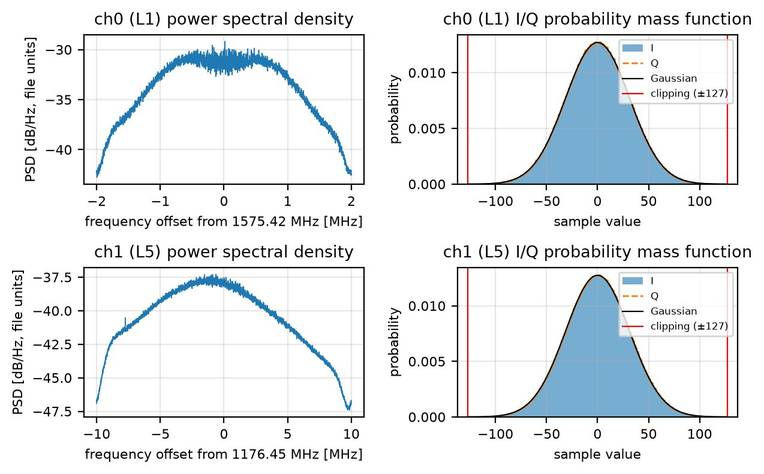
\includegraphics[width=1.0\linewidth]{gnss_sdr/x310_20261026T190001Z/source.jpg}
  \caption{Signal source: power spectral density (the receiver passband over a flat thermal-noise floor; GNSS signals are below the noise, so only interference would stand out) and probability mass functions of the integer I/Q sample values (Gaussian noise, centred, not clipped).}
\end{figure}

\begin{table}[H]
  \centering
  \footnotesize
  \resizebox{\ifdim\width>\linewidth\linewidth\else\width\fi}{!}{%
  \begin{tabular}{l>{\centering\arraybackslash}p{4.2cm}>{\centering\arraybackslash}p{4.2cm}}
    \hline
    \textbf{Channel} & \textbf{ch0} & \textbf{ch1} \\
    \hline
    Frequency [MHz] & 1575.42 & 1176.45 \\
    Rate [MS/s] & 4 & 20 \\
    Format & ci8 & ci8 \\
    Bytes per complex sample & 2 (1 for I, 1 for Q) & 2 (1 for I, 1 for Q) \\
    Full scale & $\pm$127 & $\pm$127 \\
    Gain [dB] & 25 & 25 \\
    Std I / Q & 31.4 / 31.4 & 31.3 / 31.3 \\
    Mean I / Q & 0.02 / -0.15 & -0.03 / 0.04 \\
    Min / max I & -127 / 127 & -127 / 127 \\
    Min / max Q & -127 / 127 & -127 / 127 \\
    Headroom\footnotemark & 4.0 & 4.1 \\
    Clipped [\%] & 0.004 & 0.005 \\
    Lost samples & 0 & 3,287,000 \\
    \hline
  \end{tabular}}
  \caption{Signal source: sample statistics per channel (headroom: how many standard deviations of the noise fit before clipping).}
\end{table}

\footnotetext{Headroom $= A/\sigma$, where $A$ is the full scale of the sample format (127 for 8-bit, 32767 for 16-bit) and $\sigma$ the standard deviation of the I and Q samples together (both in file units, over the analysed window). For Gaussian noise, the fraction of clipped values is $2Q(A/\sigma)$, with $Q$ the Gaussian tail function: e.g. 0.003\,\% at $4.2\sigma$.}

\subsubsection{Signal conditioner}


\begin{table}[H]
  \centering
  \footnotesize
  \resizebox{\ifdim\width>\linewidth\linewidth\else\width\fi}{!}{%
  \begin{tabular}{l>{\centering\arraybackslash}p{4.2cm}>{\centering\arraybackslash}p{4.2cm}}
    \hline
    \textbf{Channel} & \textbf{ch0 (L1 C/A)} & \textbf{ch1 (L5)} \\
    \hline
    File format & ci8 & ci8 \\
    Source item type & ibyte & ibyte \\
    Data type adapter & Ibyte\_To\_Complex & Ibyte\_To\_Complex \\
    Input filter & Pass\_Through & Pass\_Through \\
    Resampling & $\times$5 zero-order hold, offline (\texttt{upsample\_iq.py}) & Pass\_Through \\
    Rate [MS/s] & 4 $\to$ 20 & 20 $\to$ 20 \\
    \hline
  \end{tabular}}
  \caption{Signal conditioner: recorded format and rate to gnss-sdr's internal \texttt{gr\_complex} stream; both bands are read in lockstep by one \texttt{Multichannel\_File\_Signal\_Source}.}
\end{table}

\subsubsection{Acquisition}
Two-dimensional search over code delay and Doppler (one channel per band dumped; the others behave alike).

\begin{figure}[H]
  \centering
  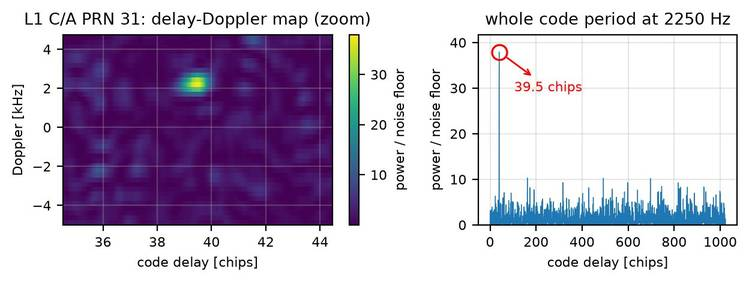
\includegraphics[width=1.0\linewidth]{gnss_sdr/x310_20261026T190001Z/acq_1C.jpg}
  \caption{Acquisition, L1 C/A: delay--Doppler search of PRN 31; one sharp peak (test statistic 51 vs threshold 47) at 2250~Hz and 39.5~chips.}
\end{figure}

\begin{figure}[H]
  \centering
  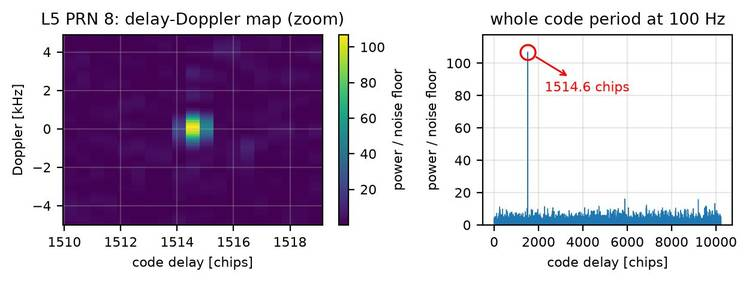
\includegraphics[width=1.0\linewidth]{gnss_sdr/x310_20261026T190001Z/acq_L5.jpg}
  \caption{Acquisition, L5: delay--Doppler search of PRN 8; one sharp peak (test statistic 148 vs threshold 49) at 1278~Hz and 1514.6~chips.}
\end{figure}

\begin{table}[H]
  \centering
  \footnotesize
  \resizebox{\ifdim\width>\linewidth\linewidth\else\width\fi}{!}{%
  \begin{tabular}{lrrrr}
    \hline
    \textbf{Band} & \textbf{Attempts} & \textbf{Detections} & \textbf{Detected PRNs} & \textbf{Best statistic / threshold\footnotemark} \\
    \hline
    L1 C/A & 3039 & 1 & 31 & 1.1 \\
    L5 & 1 & 1 & 8 & 3.0 \\
    \hline
  \end{tabular}}
  \caption{Acquisition: search attempts of the dumped channel. Attempts on satellites that are not in view (or do not broadcast that signal, e.g. older GPS satellites on L5/L2C) are rejected below the threshold.}
\end{table}

\footnotetext{Margin of the band's strongest detection: the largest acquisition test statistic among the detected attempts (the correlation peak of the delay--Doppler grid, normalised by the power of the input samples searched, i.e. the noise power, since GNSS signals are below the noise) divided by the detection threshold, which GNSS-SDR derives from the configured probability of false alarm. A value of 1 is right at the detection limit; e.g. 2.5 means the peak cleared the threshold 2.5 times over.}

\subsubsection{Tracking}


\begin{figure}[H]
  \centering
  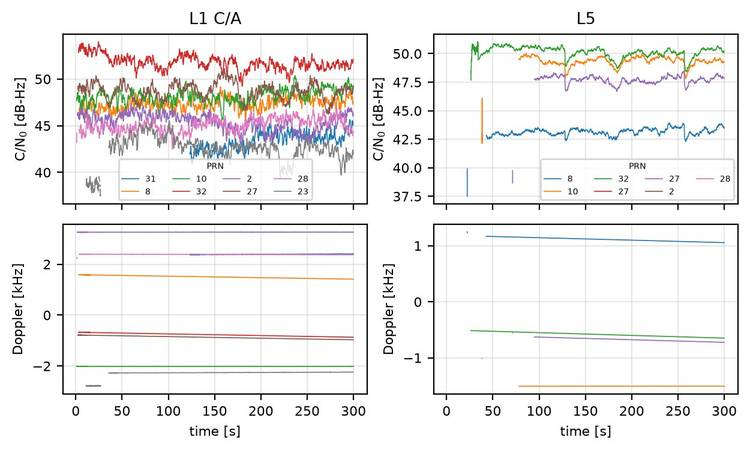
\includegraphics[width=1.0\linewidth]{gnss_sdr/x310_20261026T190001Z/tracking.jpg}
  \caption{Tracking: carrier-to-noise density ratio and carrier Doppler per satellite, while phase-locked (smooth Doppler curves = loops following the real satellite motion).}
\end{figure}

\begin{figure}[H]
  \centering
  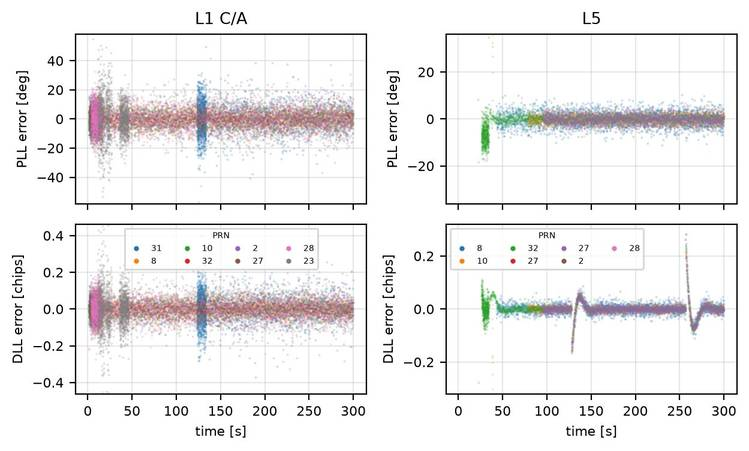
\includegraphics[width=1.0\linewidth]{gnss_sdr/x310_20261026T190001Z/tracking_errors.jpg}
  \caption{Tracking: loop errors per satellite while phase-locked, i.e. the discriminator outputs that the loops drive to zero: PLL carrier-phase error (degrees) and DLL code-delay error (chips) of every correlation. Noise centred on zero = clean tracking; its spread grows as C/N$_0$ drops, and jumps would mark cycle slips or a loop losing lock.}
\end{figure}

\begin{figure}[H]
  \centering
  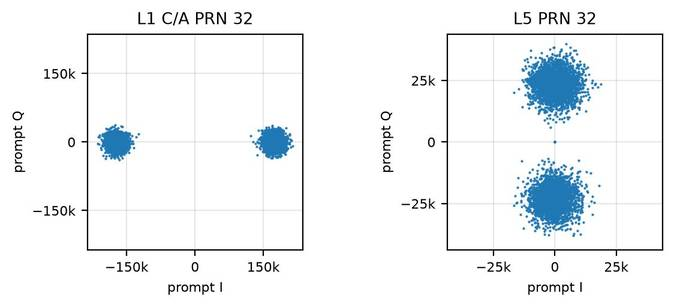
\includegraphics[width=1.0\linewidth]{gnss_sdr/x310_20261026T190001Z/tracking_iq.jpg}
  \caption{Tracking: prompt correlator outputs of the strongest satellite per band. Two tight clusters on one axis (the $\pm1$ data bits; GNSS-SDR's L5 tracking puts the data component on the Q axis), or, for the dataless pilots tracked for Galileo (E1-C, E5a-Q), the $\pm1$ chips of their secondary code, mean the PLL is phase-locked; a ring would mean it is not. \texttt{Prompt\_I}/\texttt{Prompt\_Q} are 32-bit floats (sums of the samples over one integration period, in file units): they never clip, only overflowing beyond $\pm 3.4\times10^{38}$, far above the $N\cdot\text{full scale}\cdot\sqrt{2}$ a sum of $N$ samples can reach.}
\end{figure}

\begin{table}[H]
  \centering
  \footnotesize
  \resizebox{\ifdim\width>\linewidth\linewidth\else\width\fi}{!}{%
  \begin{tabular}{lrrrrrrrr}
    \hline
    \textbf{Band} & \textbf{Ch.} & \textbf{PRN} & \textbf{Median C/N$_0$ [dB-Hz]} & \textbf{Phase-locked [\%]} & \textbf{Losses of lock} & \textbf{Tracked [s]} & \textbf{PLL error std [deg]} & \textbf{DLL error std [chips]} \\
    \hline
    L1 C/A & 0 & 31 & 42.5 & 88 & 0 & 179 & 10.5 & 0.079 \\
    L1 C/A & 1 & 8 & 47.2 & 95 & 0 & 298 & 6.3 & 0.047 \\
    L1 C/A & 2 & 10 & 48.0 & 96 & 0 & 300 & 5.7 & 0.041 \\
    L1 C/A & 3 & 32 & 52.6 & 95 & 0 & 299 & 3.5 & 0.025 \\
    L1 C/A & 4 & 2 & 46.0 & 98 & 0 & 299 & 7.4 & 0.055 \\
    L1 C/A & 5 & 27 & 49.0 & 95 & 0 & 299 & 5.1 & 0.037 \\
    L1 C/A & 6 & 28 & 44.9 & 90 & 0 & 299 & 8.4 & 0.060 \\
    L1 C/A & 7 & 23 & 42.0 & 77 & 1 & 287 & 13.4 & 0.097 \\
    L5 & 8 & 8 & 43.1 & 68 & 0 & 278 & 3.6 & 0.031 \\
    L5 & 9 & 10 & 48.1 & 34 & 2 & 278 & 2.9 & 0.029 \\
    L5 & 10 & 32 & 50.3 & 91 & 0 & 277 & 4.2 & 0.029 \\
    L5 & 12 & 27 & 28.9 & 0 & 2 & 32 & -- & -- \\
    L5 & 14 & 27 & 47.6 & 42 & 1 & 245 & 2.4 & 0.031 \\
    L5 & 15 & 2 & 28.7 & 0 & 2 & 16 & -- & -- \\
    L5 & 15 & 28 & 29.0 & 0 & 2 & 16 & -- & -- \\
    \hline
  \end{tabular}}
  \caption{Tracking: per channel and satellite (phase-locked: carrier lock test $> 0.8$; loop error standard deviations while phase-locked).}
\end{table}

\subsubsection{Telemetry decoder}


\begin{figure}[H]
  \centering
  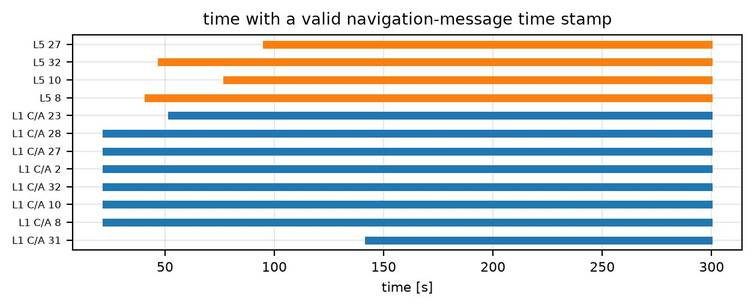
\includegraphics[width=1.0\linewidth]{gnss_sdr/x310_20261026T190001Z/telemetry.jpg}
  \caption{Telemetry decoder: per band and satellite, when the decoder delivered a valid transmit time (the first one comes after the first complete frame/message).}
\end{figure}

\begin{table}[H]
  \centering
  \footnotesize
  \resizebox{\ifdim\width>\linewidth\linewidth\else\width\fi}{!}{%
  \begin{tabular}{lrrrrr}
    \hline
    \textbf{Band} & \textbf{PRN} & \textbf{Messages decoded} & \textbf{Ephemeris} & \textbf{First valid at [s]} & \textbf{TOW [s]} \\
    \hline
    L1 C/A & 2 & 46 & yes & 21.8 & 154848.0 \\
    L1 C/A & 8 & 47 & yes & 21.8 & 154848.0 \\
    L1 C/A & 10 & 47 & yes & 21.8 & 154848.0 \\
    L1 C/A & 23 & 42 & yes & 51.8 & 154878.0 \\
    L1 C/A & 27 & 47 & yes & 21.8 & 154848.0 \\
    L1 C/A & 28 & 46 & yes & 21.8 & 154848.0 \\
    L1 C/A & 31 & 27 & yes & 141.8 & 154968.0 \\
    L1 C/A & 32 & 47 & yes & 21.8 & 154848.0 \\
    L5 & 8 & 27 & yes & 41.0 & 154867.3 \\
    L5 & 10 & 23 & yes & 76.9 & 154903.1 \\
    L5 & 27 & 21 & yes & 95.1 & 154921.4 \\
    L5 & 32 & 26 & yes & 46.9 & 154873.1 \\
    \hline
  \end{tabular}}
  \caption{Telemetry decoder: L1 C/A LNAV subframes, L5 CNAV messages decoded, ephemeris obtained, and the first valid time of week.}
\end{table}

\subsubsection{Observables}
Pseudorange, carrier phase and Doppler of every channel at common receiver epochs.

\begin{figure}[H]
  \centering
  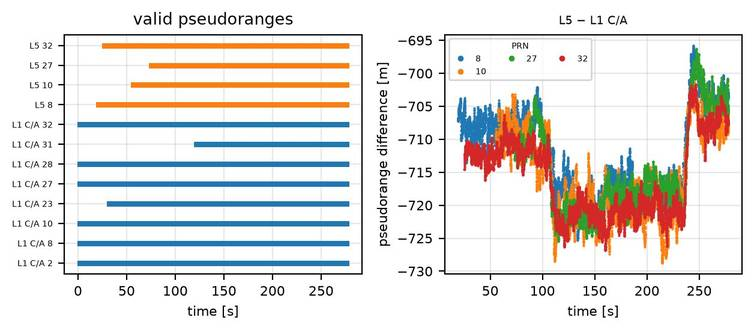
\includegraphics[width=1.0\linewidth]{gnss_sdr/x310_20261026T190001Z/observables.jpg}
  \caption{Observables: epochs with a valid pseudorange per band and satellite, and the difference between the two bands' pseudoranges of the same satellite (a constant receiver inter-band bias, the same for every satellite, plus the slowly varying ionospheric delay).}
\end{figure}

\begin{table}[H]
  \centering
  \footnotesize
  \resizebox{\ifdim\width>\linewidth\linewidth\else\width\fi}{!}{%
  \begin{tabular}{lrrrrrr}
    \hline
    \textbf{Difference} & \textbf{PRN} & \textbf{Common epochs} & \textbf{of run [\%]} & \textbf{Mean [m]} & \textbf{Std [m]} & \textbf{Drift [m/s]} \\
    \hline
    L5 $-$ L1 C/A & 8 & 12444 & 83 & -712.46 & 6.49 & -0.0031 \\
    L5 $-$ L1 C/A & 10 & 10772 & 72 & -715.60 & 6.47 & 0.0076 \\
    L5 $-$ L1 C/A & 27 & 9977 & 67 & -714.78 & 7.17 & 0.0509 \\
    L5 $-$ L1 C/A & 32 & 12166 & 81 & -715.94 & 6.04 & 0.0013 \\
    \hline
  \end{tabular}}
  \caption{Observables: pseudorange difference between the two bands of each satellite at common epochs (similar means = shared receiver bias; std = code noise of both bands).}
\end{table}

\subsubsection{PVT}
Position from the pseudoranges and the decoded ephemeris, compared with the surveyed antenna position (-23.209433$^\circ$, -45.874875$^\circ$, 596.42~m).

\begin{figure}[H]
  \centering
  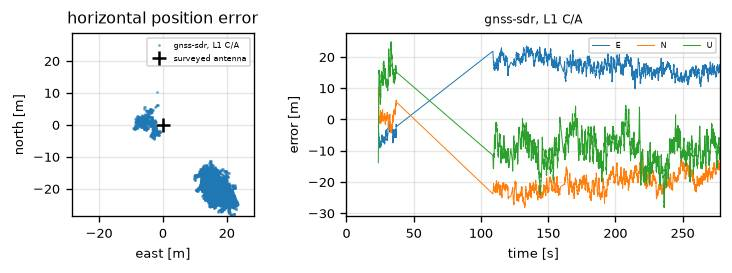
\includegraphics[width=1.0\linewidth]{gnss_sdr/x310_20261026T190001Z/pvt.jpg}
  \caption{PVT: position error of GNSS-SDR's own RTKLIB solution with respect to the surveyed antenna position (single frequency, broadcast ionosphere model).}
\end{figure}

\begin{table}[H]
  \centering
  \footnotesize
  \resizebox{\ifdim\width>\linewidth\linewidth\else\width\fi}{!}{%
  \begin{tabular}{l>{\centering\arraybackslash}p{4.2cm}}
    \hline
    \textbf{Solution} & \textbf{gnss-sdr, L1 C/A} \\
    \hline
    Solutions & 8879 \\
    Run with fix [\%] & 66 \\
    Mean E / N / U [m] & 15.2 / -18.6 / -7.8 \\
    Std E / N / U [m] & 6.3 / 6.1 / 7.9 \\
    RMS 2-D [m] & 25.6 \\
    RMS 3-D [m] & 27.9 \\
    95\% horiz. [m] & 31.8 \\
    \hline
  \end{tabular}}
  \caption{PVT: position error statistics with respect to the surveyed antenna (mean = accuracy, std = precision; \% of the run's seconds with a position; GNSS-SDR outputs several solutions per second).}
\end{table}

